% id: 33-36
% book: 베이직쎈 미적분1 · 02 함수의 연속
% section: 개념 15 연속함수
% passage: 함수 $y=f(x)$의 그래프가 다음 그림과 같을 때, 함수 $f(x)$가 주어진 구간에서 연속함수인 것은 ‘$\bigcirc$’를, 연속함수가 아닌 것은 ‘$\times$’를 (\hspace*{1.2em}) 안에 써넣으시오.
% figure: tikz:fig-33-36
% answer: 
% answer_source: 
% variant_level: 0 (원본 전사)
% 이 파일은 build.mjs 가 items.json 에서 만든다. 고칠 때는 items.json 을 고친다.
\smash{\raisebox{1.5mm}{\dmkichul{베이직쎈 미적분1 33쪽 36번}}}
\noindent\begin{minipage}[t]{0.58\linewidth}\vspace{0pt}\raggedright $[-1{,}\mkern3mu\mathopen{}1]$ \hfill (\hspace*{2.4em})\end{minipage}\hfill\begin{minipage}[t]{0.4\linewidth}\vspace{0pt}\centering \resizebox{\ifdim\width>\linewidth\linewidth\else\width\fi}{!}{% 33-36(33쪽) — 36번 그림 · y=f(x) 의 그래프(원점 대칭 쌍곡선 · x축·y축이 점근선 · (1,1), (-1,-1) 안내 점선). 스캔 화질이 낮아 TikZ 로 다시 그림.
% 원문에 있는 것만: x축 눈금 -1, 1 · y축 옆 1, -1 · 점선 네 줄 · 라벨 y=f(x), O, x, y (점 표시는 원문에 없다).
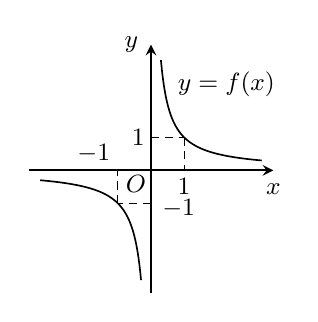
\begin{tikzpicture}[x=0.42cm, y=0.42cm, line width=0.6pt]
  \draw[->, >=stealth, line width=0.7pt] (-3.7,0) -- (3.7,0) node[below=1pt, font=\small] {$x$};
  \draw[->, >=stealth, line width=0.7pt] (0,-3.7) -- (0,3.8) node[left=1pt, font=\small] {$y$};
  \draw[densely dashed, line width=0.4pt] (0,1) -- (1,1);
  \draw[densely dashed, line width=0.4pt] (1,1) -- (1,0);
  \draw[densely dashed, line width=0.4pt] (0,-1) -- (-1,-1);
  \draw[densely dashed, line width=0.4pt] (-1,-1) -- (-1,0);
  \draw[line width=0.6pt, domain=0.30:3.35, samples=120, smooth] plot (\x, {1/\x});
  \draw[line width=0.6pt, domain=-3.35:-0.30, samples=120, smooth] plot (\x, {1/\x});
  \node[font=\small, inner sep=2.5pt, above left] at (-1,0) {$-1$};
  \node[font=\small, inner sep=2.5pt, below] at (1,0) {$1$};
  \node[font=\small, inner sep=1.5pt, below left] at (0,0) {$\pt{O}$};
  \node[font=\small, inner sep=2pt, left] at (0,1) {$1$};
  \node[font=\small, inner sep=2pt, anchor=west] at (0.15,-1.15) {$-1$};
  \node[font=\small, anchor=west, inner sep=1pt] at (0.7,2.6) {$y=f(x)$};
\end{tikzpicture}
}\end{minipage}\par
